\documentclass[11pt, oneside, a4paper]{report}  

% Input and math
\usepackage[utf8]{inputenc}
\usepackage{amsmath,amssymb,amsfonts}
\usepackage{amsthm}

% Hyperlinks
\usepackage{hyperref}

% Colors
\usepackage{color}
\definecolor{dkgreen}{rgb}{0,0.6,0}
\definecolor{gray}{rgb}{0.5,0.5,0.5}


% Source code listings (see below begindoc), graphics
\usepackage{listings}
\usepackage{graphicx}
\usepackage{subfig}
\usepackage{standalone}

\graphicspath{{Figures/}}

\begin{document}

% For source code listings
\lstset{language=Matlab,
   keywords={break,case,catch,continue,else,elseif,end,for,function,
      global,if,otherwise,persistent,return,switch,try,while},
   basicstyle=\ttfamily,
   keywordstyle=\color{blue},
   commentstyle=\color{red},
   stringstyle=\color{dkgreen},
   numbers=left,
   numberstyle=\tiny\color{gray},
   stepnumber=1,
   numbersep=10pt,
   backgroundcolor=\color{white},
   tabsize=4,
   showspaces=false,
   showstringspaces=false}

\title{Blind Source Separation}
\author{}
\date{}    % type date between braces
\maketitle

\begin{abstract}

\end{abstract}

\tableofcontents

\chapter{Introduction}

One of the many truly remarkable facet of human intelligence is our
ability to \emph{sub-conciously} process the enormous amounts
of information picked up by our sensory organs at any given moment in
time. It is worthwhile emphasizing the fact that this is a
sub-concious process, and that it takes only very little effort on the
part of the subject\footnote{One can only imagine the durdgery of life
if it were not!}. As mundane and everyday as this process may seem
then, one would expect it to be a very trivial problem. However, the
fact is quite the opposite: vast amount of effort has been undertaken in assimilating this process in
computers; some progress has been made, but we have still a long way
to go in reaching the end of human level performance in these tasks.

In this report we are to focus on a particular subset of such
filtering tasks; we are to consider audio data\footnote{It should be
 noted that many of the methods described here have been successfully
applied to visual data as well.}. Furthermore we will focus on a
particular problem known as \emph{blind source separation} (BSS). The
textbook example of BSS is the \emph{cocktail party problem} which can
be states as follows. At a fashionable cocktail party, you are
standing with fellow guests in one of several cliques, and there are
several conversations going on in the room in addition to there being
played music in the background. In this situation, you are receiving a
large number of auditory stimuli, but still you have no problem of
following the conversation in which you are parttaking. 

How is it that you are able to solve this problem so well? The human
auditory system has several clues to rely on: firstly, we are more
prone to pick up louder signals which are the voices of the people in
our proximity. Secondly, we learn quickly to recognize features such
as the pitch and loudness of the voices of those with whom you
are engaged in a conversation.

Perhaps equally important to the auditory concepts, in this setting you do not only use auditory clues in the
signal processing task -- there are also several other context
dependent pieces of information used, which in principle means that we
are not really doing truly \emph{blind} source separation. If you are discussing the various merits of
different classification algorithms you are able to follow along that
conversation because you know what type of information content such a
discussion should have. By  means of knowing such content, the brain
complements the auditory system in two ways. Firstly, you
can effortlessly ignore those behind you talking about the last
episode of Paradise Hotel, and secondly, the brain assists the
auditory system by filling in ``blanks'' if there is some word you
don't hear. Finally, we also use visual clues as a complement to
auditory functions\footnote{The best example of this is those with
  hearing impairments being able to read lips.}. 

Given the vast amount
of information we adopt as complements to the auditory system, it is perhaps no wonder that implementing this
filtering operation separately in a computer system. 

[TODO: structure of project]


\section{Formal Problem Statement}

We now provide a notation leading to a mathematical statement of the blind source separation (BSS) problem. We let $\boldsymbol{S}(t)\in \mathbf{R}^n$ for $t>0, n>0$ denote the signals generated by $n$ sources. Similarly, let $\boldsymbol{X}(t)\in \mathbf{R}^m$ for $t>0, n>0$ the observed sensor readings resulting from the emitted signals. A \emph{mixing model} $f(\boldsymbol{S},t)$ defines the relationship between source and observed signal:

\begin{equation}\label{mixing_model}
  \boldsymbol{X} = f(\boldsymbol{S},t)
\end{equation}

As only the observed value $\boldsymbol{X}$ is known, we need to determine the inverse $f^{-1}(\boldsymbol{S},t)$, that is, the \emph{unmixing model}.

\subsection*{Single Sensor Blind Source Separation}

A particular instance of the BSS problem, is the single sensor blind source separation (SSBSS) problem, to which we will devote particular attention. In the SSBSS problem, we have one or more source signals, but the observed signal $\boldsymbol{X}(t)$ is a scalar. This introduces problems as this instance does not lend itself to solutions by means of the ``standard'' methods we consider in the standard BSS problem. Chapter \ref{ssbss_chap} is devoted to the SSBSS problem.

\subsection{A Linear Mixing Model}

The simplest mixing model is a noiseless, stationary linear mixing model. The stationarity assumption means that the mixing model does not change as a function of time, so the $t$ argument in Equation \ref{mixing_model} can be omitted. With $T$ measurements, $N$ sources, and $M$ sensors, this model can be defined as:


\begin{equation}\label{linear_mixing_model}
 \boldsymbol{X} = \boldsymbol{A}\boldsymbol{S}
\end{equation}

With $\boldsymbol{}X \in \mathbf{R}^{N\times T}$, $\boldsymbol{A} \in \mathbf{R}^{N\times M}$
and $\boldsymbol{S} \in \mathbf{R}^{M\times T}$. The problem of determining the
unmixing model now consists of computing the inverse $\boldsymbol{W} = \boldsymbol{A}^{-1}$, so
that the original signal:

\begin{equation}\label{linear_unmixing_model}
\boldsymbol{S} = \boldsymbol{W}\boldsymbol{X}
\end{equation}

can be recovered. This is to say that the estimate of the original
signal $j$ at time $t$ is computed as the $j$th row of $\boldsymbol{W}$ times the
$t$th column of $X$.

From Equation \ref{linear_mixing_model}, we can see that the blind source separation problem, even in the simplest case, is ill-poised, as we are trying to determine $M\times T + N\times M$ parameters (both $\boldsymbol{A}$ and $\boldsymbol{S}$) given only $N\times T$ ($\boldsymbol{X}$). This implies that we need to impose some kind of assumptions on the nature of the data. These assumptions, often called the \emph{generative model}, state something about the nature of the signals and how they are mixed. As will be made apparent later, which assumptions are made, gives rise to different solution approaches. For the purpose of this study, we will be quite restrictive in what assumptions we are willing make, hence the term \emph{blind} source separation. The type of assumptions made are primarily related to statistical properties of the sources. The textbook assumptions are uncorrelated and independendent sources, leading to the PCA and ICA solutions, respectively\footnote{Under the assumptions that the number of observations are greater than or equal to the number of sources.}.

\section{Overview}

In the next chapters we will be looking at a few different algorithms for solving various instances of the BSS problem. Each algorithm has its own merits depending to a large extent on the assumptions we make about the data. An overview of these follow in the Table \ref{overviewTable}.

\begin{center}
  \begin{table}[h!]
    \begin{tabular}{ | l | l | l | p{5cm} |}
      \hline
      \textbf{Data characteristic} & \textbf{Method} & \textbf{Description} \\ \hline
      Uncorrelated sources. & PCA & Blabla \\ 
      Independent, non-gaussian sources. & ICA & blabla \\
      Fewer sources than observations. & HMM & blabla \\
      \hline
    \end{tabular}
    \caption{Overview over the different approaches to blind source separation covered in this report.}
    \label{overviewTable}
  \end{table}
\end{center}

\chapter{Principal Component Analysis}

Principal component analysis \cite{pearson1901} (PCA) is a eigenvector-based,
non-probabilistic technique that uses orthogonal projection to
represent data in a lower dimensional subspace spanned by the $k$
first eigenvectors of the covariance matrix. The eigenvectors form an
orthogonal basis for the data such that a projection onto the
eigenvectors will decorrelate the data. In the next section we will
derive this result by maximizing the variance of an axis of projection.

PCA is useful in several applications, hereunder visualization and
detection of so-called \emph{latent variables}. The principal
components (PCs) are the basis of the subspace onto which the data is
projected, and are such that the variance explained by each component
is maximized; that is, the first PC explains a higher proportion of
variance than the second PC and so forth. We can therefore, by
retaining only the first few components acheive a representation of
the data containing the most of the variance exhibited by the
assumption that the PCs accounting for the smallest portion of
variance are noise.


The next section presents PCA from two different but equivalent
perspectives; first solving for the direction of maximal variation
using the method of Lagrange multipliers, and subsequently by singular
value decomposition which. The latter is the more computationally
efficient, and the rationale for this approach is easy to see once the
first perspective is known. We then proceed to looking at how PCA can
be applied to the blind source problem and how the assumptions made
about the data affect the results of a real-world mixing case.


\section{Formal Statement}

Let $\boldsymbol{x}_i \in \mathbf{R}^n$ denote the $i$'th observation of a dataset
of $m$ observations. We now want to project our data onto a vector $\boldsymbol{u}$
in $\mathbf{R}^n$ so as to maximize the variance of the resulting
projection $\sum_{i=1}^m \boldsymbol{x}_i^T \boldsymbol{u}$ subject to the constraint
$|\boldsymbol{u}|=1$. Under the assumption that $\boldsymbol{X}$ is
standardized to zero mean and unit variance, the Lagrangian is then given by Equation \ref{pca_lagrangian}:

  \begin{equation}
    \label{pca_lagrangian}
    \begin{array}{lcl}
      \mathcal{L}(u,\lambda) & = & \frac{1}{m} \sum_{i=1}^m (\boldsymbol{x}_i^T \boldsymbol{u})^2 - \lambda (\boldsymbol{u}^T \boldsymbol{u} -1) \\
      \\& = & \frac{1}{m} \sum_{i=1}^m (\boldsymbol{u}^T \boldsymbol{x}_i)^T(\boldsymbol{x}_i^T \boldsymbol{u}) - \lambda (\boldsymbol{u}^T \boldsymbol{u} -1) \\
      \\& = & \frac{1}{m} \sum_{i=1}^m \boldsymbol{u}^T(\boldsymbol{x}_i \boldsymbol{x}_i^T)u - \lambda (\boldsymbol{u}^T \boldsymbol{u} -1) \\
      \\& = & \frac{1}{m}  u^T\sum_{i=1}^m(\boldsymbol{x}_i \boldsymbol{x}_i^T)\boldsymbol{u} - \lambda (\boldsymbol{u}^T \boldsymbol{u} -1) \\
      \\& = & \frac{1}{m} \boldsymbol{u}^T \boldsymbol{\Sigma} \boldsymbol{u} - \lambda (\boldsymbol{u}^T \boldsymbol{u} -1) \\
    \end{array}
  \end{equation}

Here, $\boldsymbol{\Sigma} = \sum_{i = 1}^m \boldsymbol{x}_i \boldsymbol{x}_i^T$ is the covariance matrix. Setting the gradient of \ref{pca_lagrangian} equal to zero yields Equation \ref{pca_gradient}:

\begin{equation}
  \label{pca_gradient}
  \nabla_u \mathcal{L}(\boldsymbol{u}, \lambda) = \boldsymbol{\Sigma} \boldsymbol{u} - \lambda \boldsymbol{u} = 0
\end{equation}

Equation \ref{pca_gradient} shows that the direction of maximum variance $u$, which we will refer to as the first principal component, is the first eigenvector of the covariance matrix of the dataset. By similar means it can be shown that the second eigenvector points in the direction of largest variance \emph{orthogonal} to the first eigenvector and so forth. Finally it is worth noting that the portion of the total variance explained by a principal component is proportional to its associated eigenvalue.

\subsection{Singular Value Decomposition}

For a high dimensional dataset (e.g. $n = 10,000$), which is
frequently the case working with for instance image or video data, the covariance matrix will have $10,000\times 10,000 = 100,000,000$ entries, which is computationally untractable. Hence, PCA is usually implemented in terms of \emph{singular value decomposition} (SVD). For an $m\times n$ matrix $\boldsymbol{X}$, the SVD is a factorization such that:

\begin{equation}
  X = US V^{T}
\end{equation}

Here, $U \in \mathbf{R}^{m\times m}$, $S \in \mathbf{R}^{m\times n}$,
and $U \in \mathbf{R}^{n\times n}$. The SVD relates to the eigenvalue
problem (Equation \ref{pca_gradient}) as follows:

\begin{itemize}
\item The columns of $U$ form the projections of $X$ onto the
  eigenvectors $V$.
  \item The entries $s_{ii}$ on the leading diagonal of $S$ are the
    eigenvalues of $\Sigma = X^TX$.
  \item The top $k$ columns of $V$ are the top $k$ eigenvectors of
    $\Sigma = X^T X$
\end{itemize}

In \textsc{Matlab}, we can perform SVD by a single line of code
(subsequent to standardizing the data to zero mean and unit variance):

\begin{figure}[!htpb]
  \begin{lstlisting}[frame=single]
   [U,S,V] = svd(X' * X);
  \end{lstlisting}
  \caption{\textsc{Matlab} code for SVD.}
  \label{svd_code}
\end{figure}

We will not go into the derivation of this result as SCD is covered
in most textbooks on linear algebra or basic numerical
mathematics. Rather, we will proceed to show how PCA can be applied to
BSS, and what assumptions it requires us to make about the data.



\section{PCA Application to Blind Source Separation}\label{pca_bss}
% TODO: update graphs to newest version

The top graph of Figure \ref{pca_time_series} shows two periodic signals $s_1$ and $s_2$ contaminated by an additive Gaussian white noise with standard deviation $\sigma = .2$.

\begin{equation}
      \begin{array}{lll}
        s_1 = & \sin(\pi x) & 0<x<5\\
        s_2 = & \cos(7 \pi x) & 0<5<x\\
    \end{array}
\end{equation}

The signals are subsequently mixed, as shown in the middle part of Figure \ref{pca_time_series} by the matrix:

\begin{equation}
  A = \begin{bmatrix} \cos \alpha & -\sin \alpha \\ \sin \alpha & \cos \alpha \end{bmatrix}
\end{equation}

where $\alpha = \pi/4$. Here the mixing matrix $A$ corresponds to a rotation operator that will rotate the data by $\alpha$ radians in counterclockwise direction. 

The lower part of Figure \ref{pca_time_series} shows the recovered signal\footnote{The estimated unmixing matrix here is $\hat{W} = \hat{A}^{-1} = \begin{bmatrix} .7071 & .7071 \\ -.7071 & .7071 \end{bmatrix}$ which is, as expected, the inverse of $A$ for the value of $\alpha$ above.}.

\begin{itemize}
  \item Example where it works - why
  \item Example where it fails - why
\end{itemize}



\begin{figure}
  \centering
  \hrule
  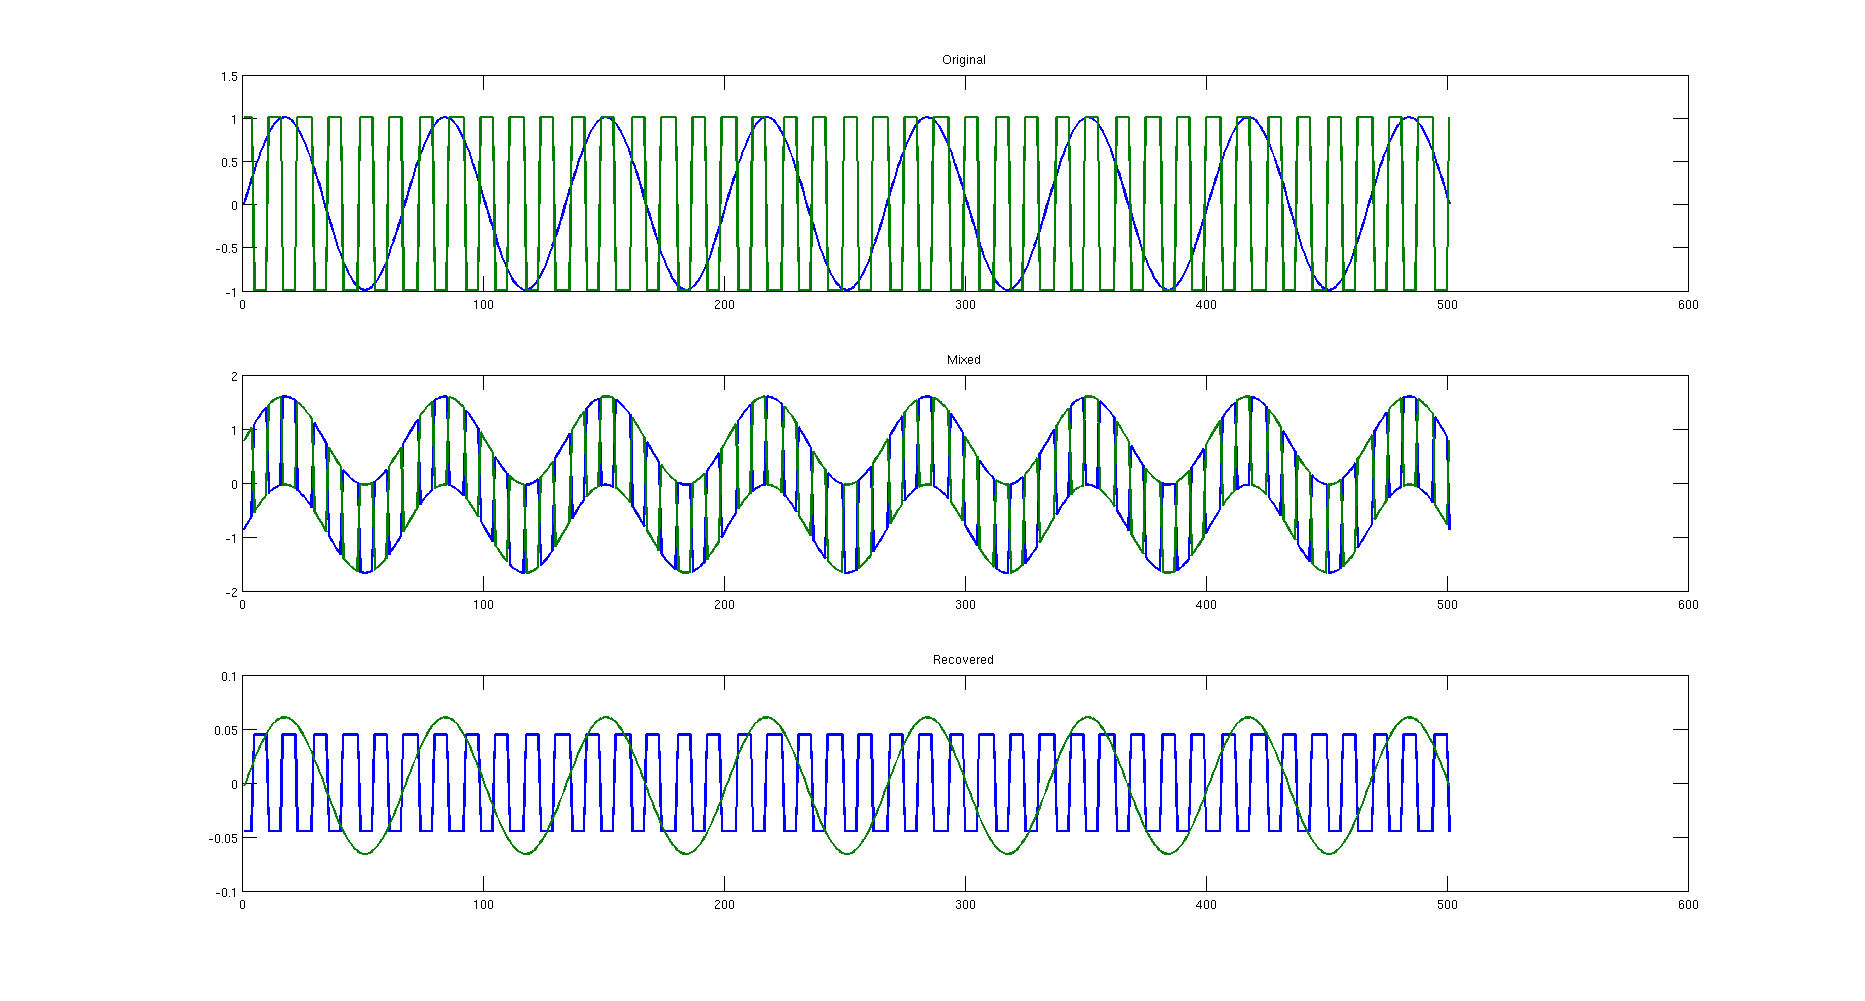
\includegraphics[width = .9\textwidth]{Figures/pca_signal_time_series}
  \hrule
  \caption{PCA Source Separation.}
  \label{pca_time_series}
\end{figure}

\begin{figure}
  \centering
  \hrule
  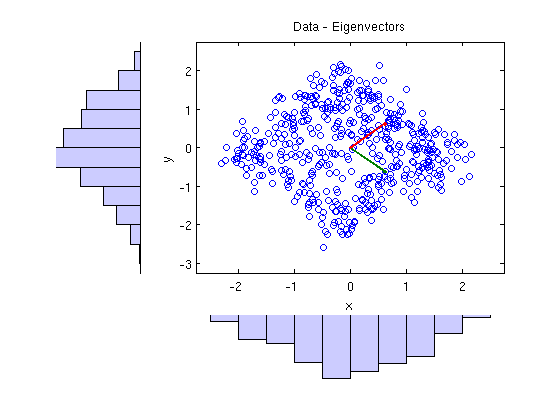
\includegraphics[width = .9\textwidth]{Figures/pca_data_eigs}
  \hrule
  \caption{Standardized data points vs eigenvectors.}
\end{figure}

\begin{figure}
  \centering
  \hrule
  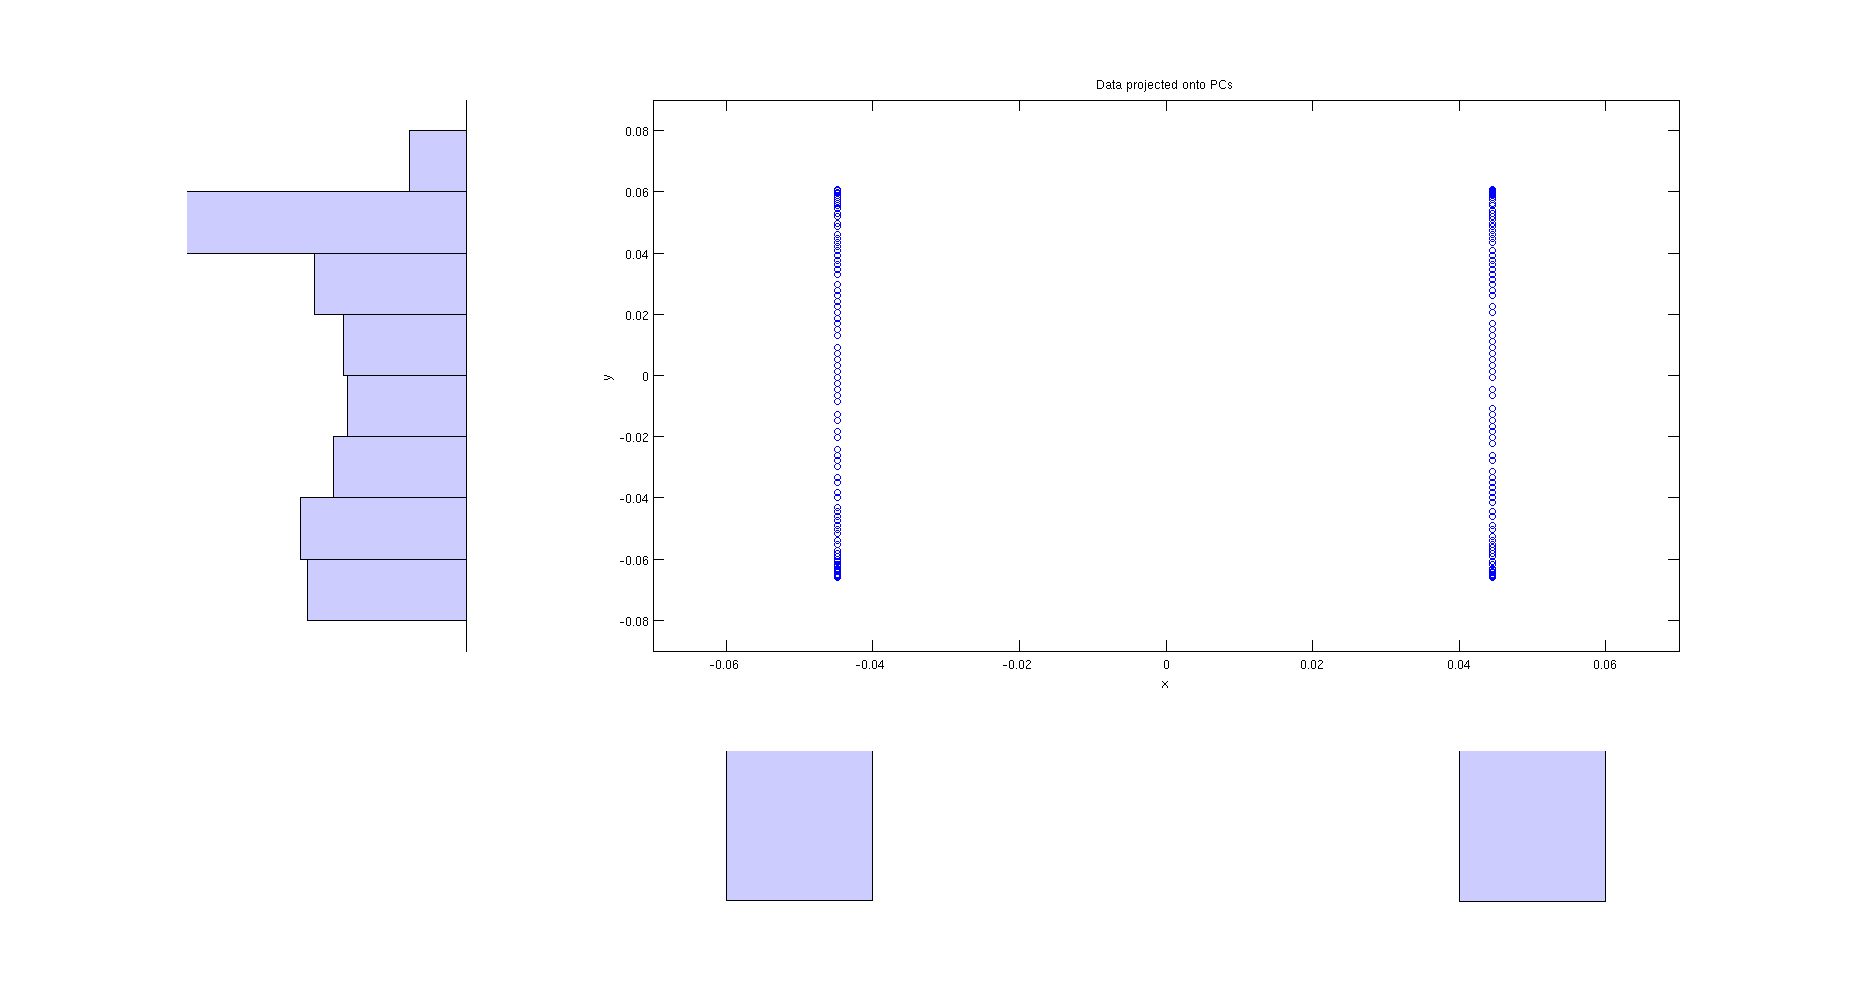
\includegraphics[width = .9\textwidth]{Figures/pca_eig_projection}
  \hrule
  \caption{Standardized data projected onto eigenvectors.}
\end{figure}

\chapter{Independent Component Analysis}

PCA finds the basis of a subspace in which the variance is
maximized in the direction of the basis vectors and the covariance
between the data is zero. ICA seeks to find basis
vectors that are statistically independent, which is a stronger
property than simply being uncorrelated as independence implies
uncorrelatedness, while the opposite is not true. ICA in contrast to PCA does not have analytic solutions in the general case, 
so a numerical optimization method is usually applied in computing the ICA transform.

\section{Limitations of the ICA Model}\label{ICA_restrictions}

ICA imposes a few critical assumptions about the nature of the sources
and the extentent to which they can be recovered. As in PCA, we cannot
recover the original ordering of the signals; i.e. the rows of the
source matrix $\boldsymbol{S}$ may be swapped in the resulting
$\hat{\boldsymbol{S}}$. Furthermore, the correct scaling of the source
compents, including their sign cannot be recovered. This can be seen
in that $\boldsymbol{X} = \boldsymbol{A}\boldsymbol{S} = (.5
\boldsymbol{A})(2 \boldsymbol{S})$.

The final limitation of ICA is that the source signals must be
non-Gaussian. To see why this must hold, we rely on the fact that the
multivariate gaussian distribution is rotationally symmetric, and that
to fully recover the sources, we must be able to ``undo'' any rotation
caused by applying the mixing operator. Consider a single observation
$\boldsymbol{x} = \boldsymbol{x}(t) =\boldsymbol{A}\boldsymbol{s}(t) = \boldsymbol{A}\boldsymbol{s}$. The covariance matrix of $\boldsymbol{x}$ is 

    \begin{equation}
      \mathbb{E}(\boldsymbol{x}\boldsymbol{x}^T) = \boldsymbol{A}\boldsymbol{s}(\boldsymbol{A}\boldsymbol{s})^T = \boldsymbol{A}\boldsymbol{s}\boldsymbol{s}^T\boldsymbol{A}^T=\boldsymbol{A}\boldsymbol{A}^T      
    \end{equation}

Now, let $\boldsymbol{R}$ be a rotation operator and $\boldsymbol{A}' = \boldsymbol{AR}$.




% \begin{itemize}
%   \item Non-Gaussian..
%   \item Ordering of signals..
%   \item ``Sign reversal'' (rotational invariance??)..
%   \item Blabla..
% \end{itemize}


\section{ICA in the Linear Mixing Model}

\subsection{Equivalent Specifications of ICA}

ICA can be derived by several different approaches:
\begin{itemize}
  \item Maximum likelihood
  \item Kurtosis maximization
  \item Maximum differential entropy
  \item Blabla..
\end{itemize}



\subsection{Derivation of ICA Log Likelihood Function}\label{ml_ica}

Let $p_s(s_i)$ be the probability density function for source $i$, then, assuming the sources are independent the joint distribution of all the $n$ sources is given by the product of the marginals:

\begin{equation}
  p(s) = \Pi_{i=1}^n p_s(s_i)
\end{equation}

We now substitute in the unmixing model (Equation \ref{linear_unmixing_model}) and obtain:

\begin{equation}
  p(s) = \Pi_{i=1}^n p_s(WX) \cdot |W|
\end{equation}

The unmixing matrix is the target parameter of our maximum likelihood approach. That is, we seek set the coefficients of the unmixing matrix so as to maximize the likelihood of observing the actual data. If our dataset consists of $T$ observations $X = \{x_1,x_2,...,x_T\}$, the log-likehliood function is:

\begin{equation}\label{ica_loglikelihood}
  l(W) =\log Prob(X|W)= \Sigma_{t=1}^T \log p_s(WX)+\log |W|
\end{equation}

As the ICA is incompatible with a Gaussian source distribution, common choices for specifying $P_s$ include the sigmoid $p_s(s) = \frac{1}{1+e^{-s}}$ and hyperbolic tangent ($\tanh(s)$).

\subsection{Derivation of Stochastic Gradient Descent for ICA}

Given the log likelihood function of Equation \ref{ica_loglikelihood},
we will now show how this can be maxmimized by stochastic gradient
descent. This derivation leads directly to a working \textsc{Matlab}
implementation shown in Figure \ref{ica_listing}.


\begin{figure}[!htpb]\label{ica_listing}
  \begin{lstlisting}[frame=single]
for i = 1:Niter
  w = update(x,w);
end

function w = update(x,w)
  x=x(:,perm);
  t=1;
  noblocks=fix(P/Blocks);
  BlocksI=Blocks*Id;
  for t=t:Blocks:t-1+noblocks*Blocks,
   u=w*x(:,t:t+Blocks-1); 
   w=w+alpha * ( BlocksI + ...
     (1-2*(1./(1+exp(-u))))*u') * w;
 end
end
  \end{lstlisting}
  \caption{\textsc{Matlab} code for ML ICA by stochastic block gradient descent.}
  \label{mlica_code}
\end{figure}



\subsection{Preprocessing}\label{ica_preprocessing}

Whitening transform...

STFT?

\section{BSS by ICA}\label{BSS_ICA}


\begin{figure}
  \centering
  \hrule
  \includegraphics[width = .9\textwidth]{Figures/ica_simple}
  \hrule
  \caption{ICA on a $2\times 2$ BSS problem. Note the ``sign reversal'' for the blue sine wave (cf. Section \ref{ICA_restrictions}).}
\end{figure}

\begin{figure}
  \centering
  \hrule
  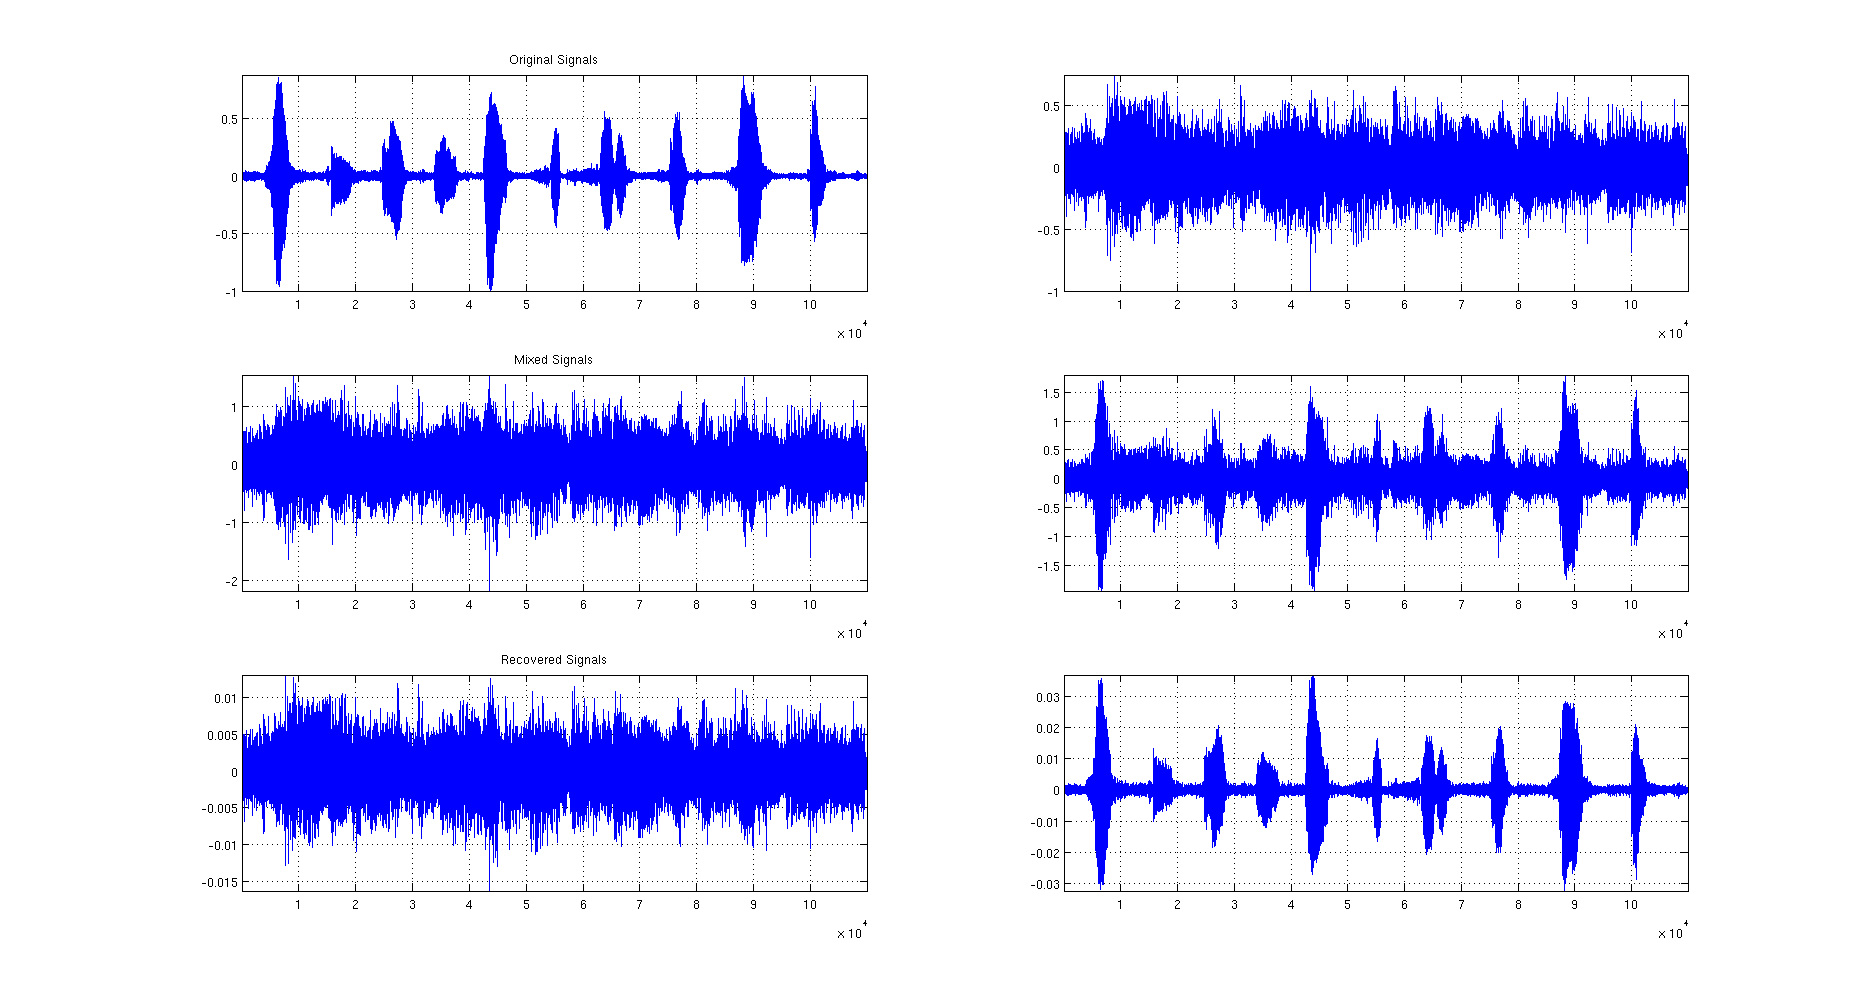
\includegraphics[width = .9\textwidth]{Figures/ica_music_speech}
  \hrule
  \caption{Separating a speech signal (top left) from background music (top right) by ICA. Here we also observe that the sign of the original speech signal is reversed in the bottom right recovered signal. }
\end{figure}




\section{Limitations and Comparison with PCA}\label{ica_conclusions}

Refer to section \ref{pca_bss} in discussion.


\chapter{Single Sensor Blind Source Separation}\label{ssbss_chap}

Single sensor BSS\footnote{Also called single channel BSS.} is a
particularly importnat case of the BSS problem where the observed
signal consists of only a scalar value at any point in time as if the
source signals were recorded a sole microphone. This presents us with
particular challenges, and we often need to make further assumptions
about the data generating process -- i.e. we need a more complex
generative model.

In this chapter we present  a solution to the single sensor BSS
problem proposed by Roweis (XXXX)\cite{roweis} that relies on a
factoral hidden markov model system. The key idea put forward by
Roweis is to learn the transition and sensor models for every source
separately using a time-frequency  representation of the original signal.

This chapter is structured as follows. Section \ref{timeFreqRep}
provides an introduction to the time-frequency domain signal
representation which is common in most single channel audio separation
models. Section \ref{fhmm} then describes the factoral hidden
markov for blind source separation in terms of a two signal mixture
before we conclude by looking at some results from our implementation
of the model.


\section{Time Frequency Signal Representation}\label{timeFreqRep}
A time frequency representation (TFR) is a redundant signal
representation in comparison to a simple time domain representation that
contains only the amplitude values at given point in time. A TFR
is often preferred to a perfect frequency or Fourier
domain representation as the latter contains no information about the
temporal location of events.


%% \begin{figure}[!htpb]\label{matlab_stft}
%%   \begin{lstlisting}[frame=single]
%% window = 256; noverlap=250; nfft=256; Freq = 16000;
%% [S,F,T,P] = spectrogram(s1,window,noverlap,nfft,Freq);
%%   \end{lstlisting}
%%   \caption{\textsc{Matlab} code for computing the short term Fourier
%%     transform of a signal sampled at $16$kHz with given
%%     parameter. P is here the power spectral density (PSD) of
%%     the signal.}
%%   \label{mlica_code}
%% \end{figure}

[....]

\section{A Latent Variable Model for BSS}

Before proceding to the full FHMM model, we will consider a simpler model without the temporal dynamics given by the markov transition model. While we are essentially dealing with a \emph{two-level latent variable model}, we follow standard terminology, adopting the term \emph{factoral-max vector quantizer} or MAXVQ for this class of models. This will also provide a ground for discussing the complexity issues of traditional inference methods as pertains to BSS, and a proposed solution to these problems.

\subsection{Generative Model and Estimation}

Let $\mathcal{Q} = \{q_1, q_2, .. , q_M\}$ denote the set of speakers\footnote{For simplicity, we assume $M=2$.}, and $Q$ be a multinomial random variable over $\mathcal{Q}$, $\mathcal{Z}_m  = \{z_1^m, z_2^m, .. , z_N^m\}$ be the set of states for the latent variable $Z^m$ for source $m$. Finally, we let $\mathbb{x} = (x_1,x_2,...,x_D)$ be an \emph{observed} $D$-dimensional frequency vector. The generative model for a given frequency band $d$ is then:

\begin{equation}
  \label{maxvq_eqn}
  \begin{array}{lcl}
    \mathbf{P}(q)   = Mn_M(q) \\
    \mathbf{P}(z|q) = Mn_N^q(z) \\ 
    z^d_{max} = \max_mz_{md} \\
    \mathbf{P}(x_d|z) = \Phi(x^d|z^d_{max},\sigma) \\
  \end{array}
\end{equation}

where $Mn_M(\cdot)$ refers to an $M$-valued multinomial distribution, and $\Phi(\cdot|\mu,\Sigma)$ the normal distribution. The idea can be expressed as follows: \emph{Each source $m$ selects a latent variable $z$ which in turn produces an intensity vector $\mathbf{x}_m$ according to the distribution $\mathbb{P}(\mathbf{x}|z)$. The final output $\mathbf{x}$ is the elementwise maximum over all vectors $\{\mathbf{x}_1, \mathbf{x}_2, ..., \mathbf{x}_M\}$}.

The model is trained in an unsupervised manner by estimating a gaussian mixture to a training dataset where sources are separated. More recently, attempts have been made at estimation directly on mixed signals [REFERANSE]. The canonical training method used in these models is the expectation maximization (EM) algorithm as described in appendix [[[REF]]]. 

\subsection{Inference}

The purpose of the inference part of the model is computing the most
likely sequence of source/gmm component combinations given the
observed data. By the log-max principle, we assume that only one
source is active at a given point in time, and for each source, we
assume there is a single maximum likelihood component. In principle, this problem could be solved by straight
forward application of the EM algorithm. This, however, is not the
preferred approach in practice because of the large state space; hence
we apply a pruning algorithm instead.

Since computing joint probabilities over the latent variables given the
observed $x$ is clearly  untractable, we look to the issue of
computing the maximum aposteriori probability (MAP) estimate of the
latent variables given the observed. To reduce the model complexity,
Roweis [[xxx]] describes a branch-and-bound procedure based on
estimating an upper ound on the log likelihood of the latent variables
given the observed data.

For source/latent variable combination $(m,k)$, given each observation
vector, $\mathbf{x}$, we compute the following bound.

\begin{equation}\label{bound}
  B_{m,k} = -\frac{1}{2}\sum_d \max(x^d - v_m^d,0)^2 - \frac{D}{2}\log|D|-\log \pi_m
\end{equation}

Next, let $z_m^{*} = \arg \min B_{m,k}$, and let $l^{*}$ be
the log likelihood associated with $z_m^{*}$. For all sources $m$, we
eliminate latent variables $k$ such that $B_{mk}<l^{*}$. For the
remaining source/latent variable combinations, we evalutate the log
likelihood by the model specified in \ref{maxvq_eqn}. If a new lower
bound is discovered, we reiterate the pruning procedure, otherwise, we
compute log likelihoods until all remaining are evaluated.




%% Once we have computed the MAP (or approximate) setting
%% of z, we can use this to estimate the refiltering masking signals as
%% follows: for each (overlapping) frame of the input spectrogram,
%% set the masking signal to unity for every frequency at which the
%% output proposed by the model corresponding to the source to be
%% recovered is the maximum proposal over all models. Other fre-
%% quencies have their masks set to zero. Actual refiltering is then
%% performed by retaining the phase from the spectrogram of the
%% original (noisy/mixed) recording, applying the (binary) masking
%% signals to the log magnitude of each frequency, and reconstitut-
%% ing the clean signal using overlap-and-add reconstruction. The
%% windowing function used to compute the original spectrogram
%% must be known (or estimated) in order to remove its effect prop-
%% erly during refiltering.



\section{Factorial Hidden Markov Model for BSS}\label{fhmm}

We will now describe the factoral HMM for blind source separation as
put forward by Roweis in a two signal setting. We adopt the following
notation: for each timestep $t \in \{1,2,3,...,T\}$, $\mathbf{X}_t$
denotes the $M$-dimensional spectral vector of power spectral
intensities over the finite set of frequency values $\mathcal{F}$. We
note that while the set of frequencies are discrete, the intensities
$x_{it}$ are real-valued, hence we adopt a real valued emission
model, as discussed later. 


\begin{figure}
  \centering
  \hrule
  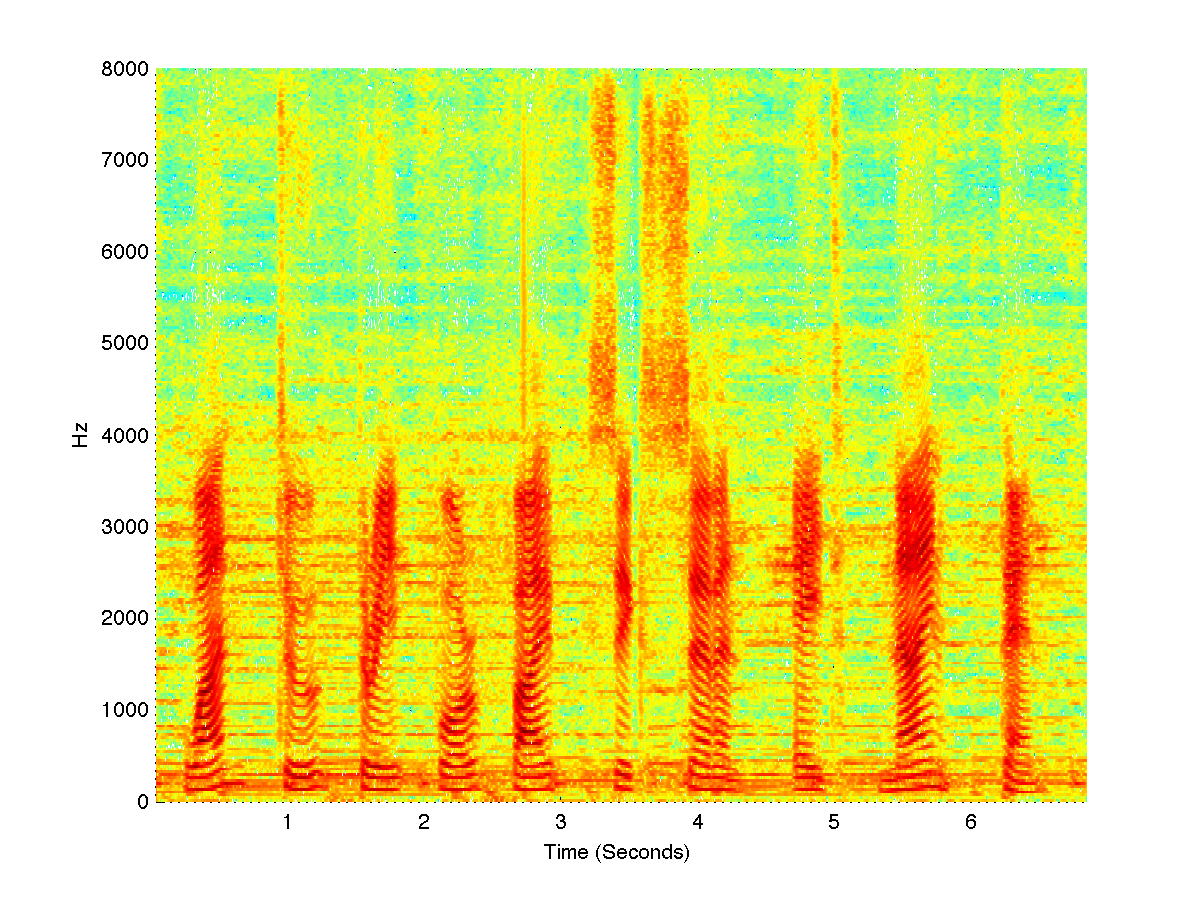
\includegraphics[width = .9\textwidth]{Figures/spectrogram_count}
  \hrule
  \caption{Spectrogram of male voice counting from one to ten.}
\end{figure}


The FHMM is essentially a supervised learning method, and the learning
process consists in estimating a separate HMM based on separate (clean) recordings of the
particular source. That is to say, the learning part consists entirely
in learning a probability model of each source. 

For a given source, the training phase then consists in
training a HMM with a discrete (latent) state space $\mathcal{Z}$, and
a continuous emission distribution $\mathbf{P(X|Z)}$. The emissions
model will produce intensity vectors $\mathbf{X}_t$ as described in
the preceding paragraph.



\subsection{Initialization}

The factoral hidden markov model consists of one HMM per speaker which
is trained on separate non-mixed training data for each source. 

The initialization of the FHMM training consists in estimating the
emission probabilities $P(X|Z)$ (see figure, lag figur). While Roweis
operates with a finite state model for the latent variables, the
observable variables are real valued intensities. This indicates that
a mixture model may be appropriate in the inital estimate of the
emission model (vis til andre artikler med samme greier ). 

We follow Roweis in estimating a Gaussian mixture model with a single
shared covariance matrix $\mathbf{\Sigma}$. For a spectrogram with $N$ frequency bands,
our approach is to estimate a GMM with $k$ $N$-dimensional components
or latent variables. The mean vector $\mathbf{\mu}_i\in\mathbb{R}^N$ for
each component $i$ represents the expected intensity (power spectral
density value) in each frequency band given that the system is in
state $i$. The pair $(\{\mathbf{\mu}_i\}, \Sigma)$ then forms the initial
parametrization of the emissions model.

\subsection{Separation}

Next, consider the problem of recovering the orignial
sources\footnote{For simplicity, we will here frame the problem in
  terms of two sources.} $\mathbf{S} =
\{S_1, S_2\}$ given the observed sequence $\{\mathbf{Y}(t)\}$, $t \in \{1,2,3,...,T\}$ which we
take to be spectral vectors as discussed above. As before, we let
$z_k(t)$, $i \in \{1,2\}$ denote the value of the latent variable for
each HMM. 

A key question in the separation process is how the observable signal
generated by full FHMM relates to the observable values for each of
the underlying HMMs. This question adresses a property of the
\emph{data generating model}, and must reflect properties of the
physical system we are trying to model. In the case of auditory
signals, Roweis argues for model whereby the observed value equals the
maximum value of the observable values $\mathbf{X}_k(t)$ of the
underlying HMMs with an additive gaussian noise:


\begin{equation}
  \mathbf{Y}(t) = \Phi(\{\mathbf{X}_1(t), \mathbf{X}_2(t)\}^{+}, \Sigma)
\end{equation}

For a further discussion on the rationale behind the log-max
approximation, see [REFERANSER].




\section{Results}



\chapter{Conclusion}

todo.

\appendix

\chapter{Literature Review}
%SLR
\documentclass[11pt, oneside, a4paper]{article}  

% Input and math
\usepackage[utf8]{inputenc}
\usepackage{amsmath,amssymb,amsfonts}
\usepackage{amsthm}

% Hyperlinks
\usepackage{hyperref}

% Colors
\usepackage{color}
\definecolor{dkgreen}{rgb}{0,0.6,0}
\definecolor{gray}{rgb}{0.5,0.5,0.5}


% Source code listings (see below begindoc), graphics
\usepackage{listings}
\usepackage{graphicx}
\usepackage{subfig}

\begin{document}

% For source code listings
\lstset{language=Matlab,
   keywords={break,case,catch,continue,else,elseif,end,for,function,
      global,if,otherwise,persistent,return,switch,try,while},
   basicstyle=\ttfamily,
   keywordstyle=\color{blue},
   commentstyle=\color{red},
   stringstyle=\color{dkgreen},
   numbers=left,
   numberstyle=\tiny\color{gray},
   stepnumber=1,
   numbersep=10pt,
   backgroundcolor=\color{white},
   tabsize=4,
   showspaces=false,
   showstringspaces=false}

\title{Blind Source Separation\\--\\A Literature Review}
\author{Anders Røsæg Pedersen\\Ulf Nore}
\date{NTNU, Fall 2012}    % type date between braces
\maketitle

\begin{abstract}
Blabla..
\end{abstract}

\tableofcontents

\section{Introduction}

The blind source separation problem refers to the process of
recovering one or more signals that have been mixed in some unknown
manner and possibly also contamined by noise. Without any assumptions
on the mixing process, this problem is ill-poised. In practice
therefore, all BSS methods rely on some stylized fact about the nature
of the signals and/or the mixing process. It is therefore useful to
dichotomize BSS methods by these assumptions.


Arguably, two of the most important facts characterizing a mixing
process, are its temporal dynamics and the number of degrees of
freedom. The first point refers to whether the nature of the mixing
process changes over time, that is if the mixing matrix at time $t+k$
is different from that at time $t$ for $k>0$. The number of degrees of
freedom is the same concept as in linear algebra - the connection is
apparent by seeing the mixing process as a system of linear
equations. If $m$ is the number of observed signals and $n$ the number
of sources, the system is said to be \emph{underdetermined} if $m<n$
and conversely \emph{overdetermined} if $m>n$. 

\begin{figure}
  \centering
  \hrule
  \includegraphics[width = .9\textwidth]{ica_simple}
  \hrule
  \caption{Stationary linear mixing process and separation.}
  \label{pca_time_series}
\end{figure}

We can also differentiate between method based on the nature of input
data. Early BSS research often considered the case of $n=m$, which
allows one to work with data in the time domain. For undetermined
systems, it is commonplace to work with some transformation of the
data, which in the case of audio data a time-frequency
representation. Common methods include the \emph{short-term Fourier
  transform} and the \emph{wavelet transform}.


The organization of this study is as follows. Section
\ref{reviewProcess} will briefly summarize the literature review
process, which is further documented by the underlying research
protocol given in Appendix \ref{protocol}. Section \ref{overview} is
an 

\section{Literature Review Process}\label{reviewProcess} % Anders



\section{Literature Overview}\label{overview}



\subsection{Independent Component Analysis} %% Ulf

%% Standard ICA
Among the most common approaches to blind source separation is
independent component analysis (ICA). Common definitions of ICA use
either the maximization of independence or minimization of mutual information between the source
signals\footnote{It should be noted that while this text presents ICA
  in terms of blind source separation, the method is applicable to a
  wide array of machine learning problems including dimension
  reduction, classification, and de-noising.}. Formally, we can state
the ICA problem in terms of a generative model of the observed signals
$\mathbf{x}$, and the unknown a mixing matrix $\mathbf{W}$ and source
signals $\mathbf{s}$:


\begin{equation}
  \mathbf{x} =   \mathbf{W}  \mathbf{s}
\end{equation}

The AIM of the ICA process is to estimate the inverse mixing process
along with the original signals.

The classical reference on ICA
is \cite{comon94}, where the method of minimization of mutual
information between sources is presented. \cite{comon94} also presents an
analysis of the ambiguities and limitations of ICA, hereunder the permutation of
sources, scaling and non-gaussianity. 

There are several equivalent statements of ICA, which yields different
interpretations and computational models.
\cite{bellSejnowski95} proposes minimizing mutual information between
sources, as measured by \emph{differential entropy}. In this
implementation a feed-forward neural network structure is proposed.
Other approaches include conventional maximum likelihood (\cite{pearlmutterParra}) and maximization of
non-gausianity as measured by excess kurtosis. A popular approach is
the  FastICA algorithm (\cite{fastICA}) that minimizes mutual
information expressed by \emph{negentropy} by a fixed point method. 

The classic studies on ICA focus to a large extent on developing the
formal framework for ICA, and examples are largely centered on time
domain analysis in systems of an equal number of sensors and
sources\footnote{For a much more thorough survey on the classical literature 
on ICA, see \cite{hyvarinen2001}.}. ICA has however been extended to underdetermined systems and
the extreme case of single sensor systems. 

Many of these extensions are to a lesser extent changes to the
previously known algorithms; rather they involve transforming
the observed signals from the time domain to some other basis, the
most common of which are the frequency domain (Fourier transform), the
time-frequency domain (short-term Fourier transform) and the wavelet
domain. Compared to the time domain, the two latter are redundant
representations, but they transform the data so as to be suited for
ICA. \cite{mijovic2010} surveys variations on ICA as applied to single
channel recordings, hereunder single channel ICA (SCICA) and wavelet
ICA (WICA), in addition to proposing an algorithm that combines ICA
with empirical mode decompostion (EMD). EMD decomposes a signal into
independent components in the spectral domain and can be viewed as
similar to STFT.

The abovementioned approaches represent a select set of common
approaches to the  BSS problem. Other approaches rely to a larger
extent on direct application of knowledge about the human auditory
system. As an example \cite{bach} focuses on the problem on single channel speech
separation in the spectral domain by means of feature
maps where the features roughly corresponds to ``audible'' features such
as common onset, pitch, timbre and so forth. 

\begin{table}[position specifier]
  \centering
  \begin{tabular}{|l|l|l|p{5cm}|}
    \hline
    \textbf{Study} & \textbf{Method} & \textbf{Data} & \textbf{Description} \\
    \hline
    Comon (94) & ICA & Time domain & Blabla.. \\
    Bell and Sejnowski (95) & ICA & Time domain & Joint entropy
    maximization by gradient descent.\\
    Hyvarinen (01) & FastICA & Time domain & Fixed point negentropy
    minization \\
    Roweis (01) & Factoral HMM & Time-frequency domain & Masking signals on frequency spectrum  \\

    \hline
  \end{tabular}
  \caption{Overview over blind source separation methods}
  \label{tab:myfirsttable}
\end{table}


\subsection{Factoral Hidden Markov Models} %% Anders
The Hidden Markov modelling has been around since the late 1960s. Roweis\cite{roweisOneMic} proposes a technique called refiltering, where the idea is to separate sources in a mixed or corrupted recording. This is achieved through non stationary masking of the different frequency sub-bands from the target recording. Different sources may be isolated in the recording by changing the masking parameters. Using regularities in the spectrogram produced by a recording, it is possible to set the masking parameters, eg. common onset and offset.

\begin{figure}[h]
  \centering
  \hrule
  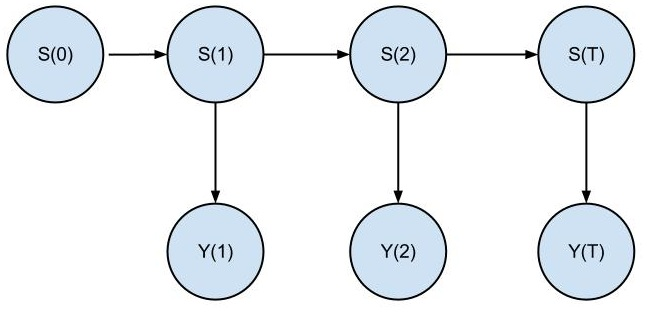
\includegraphics[width = .9\textwidth]{hmm}
  \hrule
  \caption{Hidden Markov Model}
  \label{hmm_figure}
\end{figure}



Training speaker dependent HMMs on isolated data from the sources to be separated, these models are then combined together in an architecture called factorial-max HMMs. The different HMMs evolve independently and for each observation vector produced at time t by each HMM, the elementwise maximum is chosen to create an observation. This is because the log magnitude spectrogram of a mixture of sources is very similar to the elementwise maximum of the individual spectrograms\footnote{This example was performed on two speakers. $a_{x_{t}}$ is the observation vector for speaker $x$ at time $t$, likewise is $b_{z_{t}}$ the observation vector for speaker $z$ at time $t$}. Separation is performed by setting the various masking signals to 1 or 0, depending on the observation vector at time $t$ for frequency band $i$.

\begin{figure}[h]
  \centering
  \hrule
  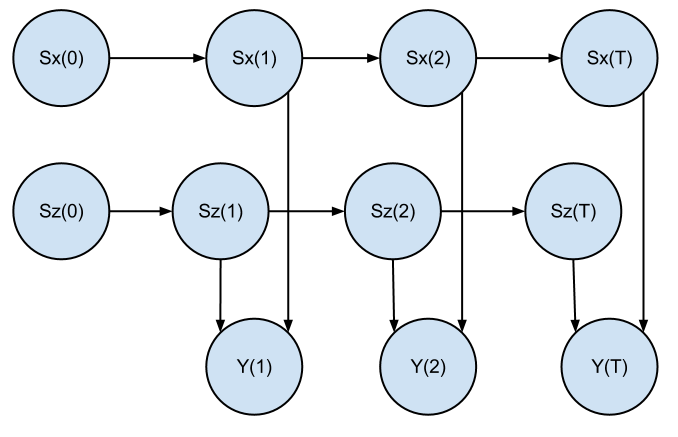
\includegraphics[width = .9\textwidth]{f_hmm}
  \hrule
  \caption{Factorial Hidden Markov Model}
  \label{fhmm_figure}
\end{figure}

The full generative model is given in Equations \ref{roweisEqn1} - \ref{roweisEqn3}.

\begin{equation}\label{roweisEqn1}
  p(x_{t}=j|x_{t-1}=i)=T_{ij}
\end{equation}

\begin{equation}\label{roweisEqn2}
  p(z_{t}=j|z_{t-1}=i)=U_{ij}  
\end{equation}

\begin{equation}\label{roweisEqn3}
  p(y_{t}|x_{t},z_{t})=N(max[a_{x_{t}},b_{z_{t}}], R)  
\end{equation}


\section{Conclusion}

In this survey we have provided an overview over some techniques in
blind source separation. Early work on blind source separation focused
to a large extent on time domain ICA. In extending the BSS problem to
multiple sources, the classical ICA method has been augmented by
adopting different signal representations, where the time-frequency
domain is particularly common. Different methods have also been
introduced, some borrowing from the human auditory system attempting
to hard-code domain specific knowledge. Others adopt different
algorithms; one important example here being hidden markov models
(HMMs). This is a very flexible approach to BSS as it allows for
non-stationary mixing, and relaxes many of the stringent assumptions
of classical ICA. 

\newpage
\appendix


\section{Research Agenda}
The aim of this study is to systematically review current technology
for blind source separation (BSS), with particular emphasis on the
particular subproblem of single channel blind source separation
(SCBSS); that is, the recovery of several source signals from one observed signals.


\subsection{Background}
The blind source separation problem consists transforming a set of observed signals that has undergone some particular mixing process back to the original unobserved signals. The “blind” part of the problem refers to the fact that the nature of the mixing process is unknown. From original research on the blind source separation problem, focus has shifted from the case where with as many, or more recording channels than original sources, to the case of fewer channels than original sources. An important subproblem that we wish to focus on is where we have only one recording and attempt to recover multiple sources.

Our approach is two-fold: firstly we wish to look at studies about the performance of current single channel separation methods. Secondly, we wish to gain a broader overview over the state of research on BSS.

\subsection{Research Questions}
\begin{enumerate}
  \item What are the different variations on the blind source
    separation problem, in particular as pertains to audio data.
  \item Which methodologies and algorithms are applied to the
    different variations of the blind source separation problem as identified in Question 1.
  \item What are the theoretical properties of the techniques
    identified in Question 2, and  what assumptions do they make about the nature of the sources and the mixing process?
  \item What empirical evidence is there to document the performance
    of the techniques identified in Question 2 as applied to the
    problems identified in Question 1?
\end{enumerate}



\subsection{Search Strategy}
In reviewing the BSS literature we conduct a search of the below databases based on a set of keywords listed below. To filter the results we introduce a set of criteria to judge the relevance and quality of the results.

\subsubsection{Databases}

\begin{itemize}
 \item \href{www.springerlink.com}{SpringerLink}
 \item \href {www.citeseerx}{CiteSeerX}
 \item \href{scholar.google.com}{Google Scholar}
\end{itemize}

\subsubsection{List of Search Terms}

\emph{blind source separation, single channel blind source separation, single mixture blind source separation, hidden markov blind source, single microphone blind source separation, blind source separation review, blind source separation survey, pca blind source separation, ica blind source separation, principal component analysis blind source separation, independent component analysis blind source separation}.



\subsubsection{Inclusion and Quality Criteria}
We wish to study how various methods and/or approaches by which blind source problem is solved, which constraints are imposed by these methods, and how well a BSS system based on these ideas perform on real-life data. To filter out the most important studies to this end, we adopt the following criteria.

\begin{description}
	\item Inclusion Criteria
		\begin{enumerate}
			\item The main concern of the study is the BSS
                          problem.
			\item The algorithmic design decisions in the study must be justified.
			\item The study describes a reproducible algorithm/method.
			\item The study focuses on blind source separation of auditory signals.
		\end{enumerate}
	\item Quality Criteria
		\begin{enumerate}
			\item The study presents empirical results.
			\item More recent studies are preferred.
			\item The described test data set is
                          reproducible.
                        \item The study should present novel
                          theoretical approaches/methodologies OR
                          empirical results about previously known methods. 
			\item Literature reviews should discuss single channel blind source separation.
			\item The study should describe which other algorithms/methods the proposed solution can be compared with and the performance measure used in comparison.
		\end{enumerate}
\end{description}

\begin{thebibliography}{99}

\bibitem{comon94} Comon, P. (1994). 
``Independent Component Analysis: a new concept?'', 
Signal Processing, 36(3):287–314

\bibitem{bellSejnowski95} Bell, A.J. and Sejnowski, T.J. (1995).,
``An information maximization approach to blind separation and blind deconvolution'', 
Neural Computation, 7, 1129-1159

\bibitem{pearlmutterParra}Pearlmutter, B. A. and Parra, L. C.(YYYY),
``A Context-Sensitive Generalization of ICA''. 

\bibitem{hyvarinen2001}Hyvarinen A (2001),
``Independent Component Analysis'',
Neural Computing Surveys, Neural Computing Surveys, vol 2.

\bibitem{bach} Bach, F.R. and Jordan, M.I. (2004),
``Blind One-Microphone Speech Separation: A Spectral Learning
  Approach''.

\bibitem{fastICA}Hyvärinen, A. (1999),
``Fast and Robust Fixed-Point Algorithms for Independent Component
  Analysis''. 
IEEE Transactions on Neural Networks 10(3):626-634, 1999.

\bibitem{roweisOneMic}Sam T. Roweis(2001).
``Neural Information Processing Systems 13'' (NIPS'00).
pp. 793-799
  
\bibitem{davies2007}Davies, M.E. and James, C.J. (2007).
``Source separation using single channel ICA'',
Signal Process., vol. 87, no. 8, pp. 1819–1832, 2007.

\bibitem{cardoso98}Cardoso, J. L.(1998),
``Multidimensional Independent Component Analysis'',
Proceedings of ICASSP 1998.

\bibitem{mijovic2010} Mijovic, B. De Vos, M.,  Gligorijevic, I.,
  Taelman, J. and Van Huffel, S. (2010),
``Source Separation From Single-Channel Recordings by Combining
  Empirical-Mode Decomposition and Independent Component Analysis'',
IEEE Transactions on Biomedical Engineering, vol. 57, no. 9, September 2010

\end{thebibliography}




\end{document}


\chapter{Mathematical Concepts}

In this appendix we will provide a brief background on some of the mathematical notions that are central to understanding the methods used in this report. 

\section{Linear Algebra}

% the easy stuff
In this section we will define a few important concepts that are
necessary. These concepts are particularly important for understanding
PCA, but are also relevant in the analysis of markov models. With
stationary transition probabilities, the steady state distribution of
the system is the solution to the eigenvector-eigenvalue problem.

\subsubsection{The Eigenvector - Eigenvalue Problem}

\subsubsection{Singular Value Decomposition}


\section{Statistics and Optimization}

% ML-estimation + gradient descent
A large portion of machine learning relies on statistical
methods; the methods considered in this report being no exception. As the learning problems having relevance in practical life are often
far too complex to describe by analytic formulae, we therefore often
need mathematical methods to find models that have the best fit to the
observed data. 

In this section, we therefore consider one very
important method for finding ``optimal'' parameters in a given model;
the maximum likelihood method which is presented in Section
\ref{ml-estimation}. We then proceed to show how to actually solve
the resulting maximzation in Section \ref{optimization}.


\subsection{Maximum Likelihood Estimation}\label{ml-estimation}

ML estimation is a method for determining the parameters of a
statistical model by setting the parameters so as to maximize the
\emph{likelihood} of observing the actual data under the given
model. Denoting $f(\boldsymbol{X}|\boldsymbol{\Theta})$ the
probability distribution of $\boldsymbol{X} = \{x_1,x_2,...,x_n\}$
with parameters $\boldsymbol{\Theta} = \{\theta_1, \theta_2, ...,
\theta_m\}$, the maximum likelihood estimate of $\Theta$ solves Equation\ref{ml-generic}

\begin{equation}
  \label{ml-generic}
  \arg \max_\Theta f(\boldsymbol{X}|\boldsymbol{\Theta})
\end{equation}

An important case is if the $x_i$ are i.i.d., where the joint density
is the product of the marginal densities. This means we can write the
likelihood function $f$ as Equation \ref{ml-iid}.

\begin{equation}  
  \label{ml-iid}
  f(\boldsymbol{X}|\boldsymbol{\Theta}) = \prod_{i = 1}^n f(x_i|\Theta)
\end{equation}

The solution to an optimzation problem is the same under any monotone transformation. Therefore it is often times useful to deal with the log-likelihood function instead of $f$ directly.


\subsection{Mathematical Optimization}\label{optimization}

\subsubsection{The Lagrange Multiplier Method}

\subsubsection{Gradient Descent}


\section{Spectral Analysis}

In working with hidden markov models for blind source separation, we
rely on a redundant signal representation in the time-frequency
domain, rather than the standard representations in the time
domain. Such a representation is advantageous in comparison with a
pure spectral representation as the latter contains no information on
when different components of a signal occur in time. While many
different time-frequency representations exist, our presentation
relies on the \emph{short-term Fourier transform} (STFT).

The time-frequency representation, often called a \emph{spectrogram} produced by the STFT maps the
energies in various parts of the spectrum over the timespan of the
signal. For a low amplitude portion of the signal will have its energy
concentrated in the upper part of the spectrogram and vice versa. This
is illustrated in Figure XX.

[[[[[[[[[[ FIGURE HERE!!! ]]]]]]]]]

\subsection{Formal statement}

Equation \ref{stft} defines the discrete time STFT for the $n$th
segment (which is centered around $m$):

\begin{equation}\label{stft}
  \text{STFT}\{x[n]\}(m,\omega)= X(m,\omega) =\sum_{n = -\infty}^{\infty}
  x[n]\omega[n-m]e^{-i\omega n}
\end{equation}

Here, $\omega$ is a zero centered window function, typically uniform
or gaussian. The window determines which part of the signal $x$ is to
be included in the spectrogram near $m$. In practice, the STFT is
computed using the fast fourier transform (FFT). To better allow for
visualization of the STFT, which is a complex number, the spectrogram
is defined as the squared magnitude of the STFD (Equation \ref{spectrogram}).

\begin{equation}\label{spectrogram}
  \text{spectrogram}\{x[n]\}(m,\omega) = |X(m,\omega)|^2 
\end{equation}


\section{Gaussian Mixture Models}\label{gmm_appendix}
A gaussian mixture model (GMM) is latent variable model that gives a
tractable representation of high-dimensional probability
distribution. Let $Z$ be a multinomial random variable taking on
values $z \in \{1,2,3,...,N\}$ and $\{X_i\}$, $i \in \{1,2,3,...,N\}$
be a set of (multivariate) Gaussian random variables. If $X$ and $Z$
har the joint distribution (\ref{gaussmix_eqn}) then we say $X$ and $Z$
has a gaussian mixture distribution:

\begin{equation}\label{gaussmix_eqn}
  \mathbb{P}(X,Z) = \mathbb{P}(X|Z)P(Z) = \sum_{i = 1}^N
  \Phi(X_i,\mathbf{\mu}_i, \mathbf{\Sigma}_i)Mn_N(Z)
\end{equation}

Here, $\Phi(X,\mathbf{\mu}, \mathbf{\Sigma})$ denotes $X$ having a
gaussian distribution with expectation vector $\mathbf{\mu}$ and
covariance matrix $\mathbf{\Sigma})$, and $Mn_N(Z)$ denotes $Z$ having
an $N$-valued multinomial distribution.

A common interpretretation of the gaussian mixture model is for $Z$ to
represent a latent or hidden variable describing the state of a
system, while $X$ is some observable quantity depending on the state
of the system. 


\section{Hidden Markov Models}\label{hmm_appendix}
%% Ref Norvig
A hidden markov model (HMM) is a probabilistic model relating two sequences of
discrete random variables $\mathcal{S} = \{S_1, S_2, ..., S_T\}$ and
$\mathcal{X} = \{X_1, X_2, ..., X_T\}$. We will refer to
$\mathcal{S}$ as the \emph{source} or \emph{hidden} variable, and
$\mathcal{X}$ as the \emph{observed} variable. Often, we assume there
is some causal relationship whereby the hidden variable affects the
observable, but this does not need be the case. 

A HMM consists of two probabilistic statement; the \emph{transition}
model:

\begin{equation}
\mathbb{P}(S_t|S_{t-1}, S_{t-2},...,S_1)
\end{equation}


and the \emph{sensor} or \emph{observation} model:

\begin{equation}
\mathbb{P}(X_t|S_t, S_{t-1}, X_{t-1}, ...,
S_1, X_1)
\end{equation}


 The order of a markov model is the number of realizations
of $\mathcal{S}$ conditioned on in the transition model. In order to
make HMMs computationally tractable, we often operate with 1st order
markov models:

\begin{equation}\label{1st_order_markov}
  \mathbb{P}(S_t|S_{t-1}, S_{t-2},...,S_1)  =  \mathbb{P}(S_t|S_{t-1})
\end{equation}

This can be stated as as ``the future being conditionally independent of
the past given the present''. Another common simplification is known as the \emph{markov sensor model assumption}:


\begin{equation}
  \mathbb{P}(X_t|S_t, S_{t-1}, X_{t-1}, ...,
  S_1, X_1) = \mathbb{P}(X_t|S_t)  
\end{equation}

The sensor markov assumption states that the sensor is independent of
everything else given the current value of the hidden variable.


\begin{thebibliography}{99}

\bibitem{comon94} Comon, P. (1994). 
``Independent Component Analysis: a new concept?'', 
Signal Processing, 36(3):287–314

\bibitem{bellSejnowski95} Bell, A.J. and Sejnowski, T.J. (1995).,
``An information maximization approach to blind separation and blind deconvolution'', 
Neural Computation, 7, 1129-1159

\bibitem{pearlmutterParra}Pearlmutter, B. A. and Parra, L. C.(1996),
``A Context-Sensitive Generalization of ICA''. 

\bibitem{hyvarinen2001}Hyvarinen A (2001),
``Independent Component Analysis'',
Neural Computing Surveys, Neural Computing Surveys, vol 2.

\bibitem{bach} Bach, F.R. and Jordan, M.I. (2004),
``Blind One-Microphone Speech Separation: A Spectral Learning
  Approach''.

\bibitem{fastICA}Hyvärinen, A. (1999),
``Fast and Robust Fixed-Point Algorithms for Independent Component
  Analysis''. 
IEEE Transactions on Neural Networks 10(3):626-634, 1999.

\bibitem{roweisOneMic}Roweis, Sam T.(2001).
``Neural Information Processing Systems 13'' (NIPS'00).
pp. 793-799
  
\bibitem{davies2007}Davies, M.E. and James, C.J. (2007).
``Source separation using single channel ICA'',
Signal Process., vol. 87, no. 8, pp. 1819–1832, 2007.

\bibitem{cardoso98}Cardoso, J. L.(1998),
``Multidimensional Independent Component Analysis'',
Proceedings of ICASSP 1998.

\bibitem{mijovic2010} Mijovic, B. De Vos, M.,  Gligorijevic, I.,
  Taelman, J. and Van Huffel, S. (2010),
``Source Separation From Single-Channel Recordings by Combining
  Empirical-Mode Decomposition and Independent Component Analysis'',
IEEE Transactions on Biomedical Engineering, vol. 57, no. 9, September 2010

\bibitem{VargaHMMDecomp}Varga, A. P., and R. K. Moore. 
``Hidden Markov model decomposition of speech and noise"
Acoustics, Speech, and Signal Processing, 1990. ICASSP-90., 1990 International Conference on. IEEE, 1990.

\bibitem{pearson1901}{Pearson, K. (1901). ``On Lines and Planes of Closest Fit to Systems of Points in Space". Philosophical Magazine 2 (6): 559–572.}

\bibitem{Pham}{Pham, D. T. and Garat, P. (1992) ``Blind Separation of Mixture of Independent Sources Through a Maximum Likelihood Approach'', Proc. EUSPICO, pp. 771-774.}

\bibitem{norvig_russel}{Russell, S. and Norvig, P. (XXX). ``Artificial
    Intelligence: A Modern Approach''. XXXX}


\end{thebibliography}








\end{document}

